\documentclass[12pt,a4paper]{article}
\usepackage[margin=1in]{geometry}
\usepackage{graphicx}
\usepackage{amsmath,amssymb}
\usepackage{booktabs}
\usepackage{multirow}
\usepackage{float}
\usepackage{listings}
\usepackage{xcolor}
\usepackage{caption}
\usepackage{subcaption}
\usepackage{hyperref}
\usepackage{enumitem}
\usepackage{fancyhdr}
\setlength{\headheight}{15pt}

% Code listing style
\lstset{
    language=C,
    basicstyle=\footnotesize\ttfamily,
    keywordstyle=\color{blue}\bfseries,
    commentstyle=\color{green!50!black},
    stringstyle=\color{red},
    numbers=left,
    numberstyle=\tiny\color{gray},
    numbersep=5pt,
    breaklines=true,
    frame=single,
    backgroundcolor=\color{gray!5},
    tabsize=4,
    showstringspaces=false,
    captionpos=b
}

% Pseudocode style
\lstdefinestyle{pseudocode}{
    basicstyle=\footnotesize\ttfamily,
    keywordstyle=\color{blue}\bfseries,
    commentstyle=\color{green!50!black}\itshape,
    numbers=left,
    numberstyle=\tiny\color{gray},
    numbersep=5pt,
    breaklines=true,
    frame=single,
    backgroundcolor=\color{yellow!5},
    tabsize=4,
    morekeywords={FUNCTION,END,PARALLEL,REGION,FOR,IF,STATIC,ALLOCATE,MEMSET,CLAMP,FLOOR},
    captionpos=b
}

\pagestyle{fancy}
\fancyhf{}
\rhead{HPC Assignment 06}
\lhead{Om Patel \& Chaitanya Vats}
\cfoot{\thepage}

\begin{document}

% ============================================================
% TITLE PAGE
% ============================================================
\begin{titlepage}
\centering
\vspace*{2cm}

{\LARGE\bfseries High Performance Computing (HPC)\\[0.3cm]}
{\Large\bfseries Assignment 06 -- Parallel Interpolation\\[1.5cm]}

\rule{\textwidth}{1pt}\\[1cm]

{\large
\begin{tabular}{rl}
\textbf{Name:} & OM PATEL \\
\textbf{Roll Number:} & 202301163 \\[0.5cm]
\textbf{Name:} & CHAITANYA VATS \\
\textbf{Roll Number:} & 202301419 \\
\end{tabular}
}

\vspace{1.5cm}

{\large Dhirubhai Ambani University \\[0.3cm]}
{\large Instructor: Dr.\ Bhaskar Chaudhury \\[0.3cm]}
{\large Teaching Assistants: Libin Varghese, Ayushi Sharma, Kaushik Prajapati \\[0.5cm]}
{\large April 2026}

\vfill
\rule{\textwidth}{1pt}
\end{titlepage}

\tableofcontents
\newpage

% ============================================================
% SECTION 1: PROBLEM STATEMENT
% ============================================================
\section{Problem Statement}

This assignment focuses on \textbf{parallelizing} a scatter point-to-mesh bilinear interpolation algorithm using \textbf{OpenMP}. MPI is not permitted for this assignment. The goal is to transform a correct serial baseline into a high-performance parallel implementation.

\subsection{Problem Description}

Given a set of $N$ scattered points in a 2D domain of size $1 \times 1$:
\[
S = \{(x_i, y_i, f_i) \mid i = 1, 2, \ldots, N\}
\]
where $(x_i, y_i)$ are spatial coordinates and $f_i = 1$ for all points. The task is to \textbf{interpolate} these values onto a structured mesh grid of size $M_x \times M_y$.

\subsection{Step-by-Step Procedure}

\begin{enumerate}
    \item \textbf{Read input data}: Load $N$ scattered points $(x_i, y_i)$ from a binary file \texttt{input.bin}. The domain is a unit square $[0,1] \times [0,1]$.
    
    \item \textbf{Initialize structured mesh}: Define the grid $G$ with $(N_x + 1) \times (N_y + 1)$ grid points and set all function values $F(X_i, Y_j) = 0$.
    
    \item \textbf{For each scattered point $(x_i, y_i)$}:
    \begin{enumerate}
        \item Identify the cell containing the point by computing:
        \[
        i = \left\lfloor \frac{x_i}{\Delta x} \right\rfloor, \quad j = \left\lfloor \frac{y_i}{\Delta y} \right\rfloor
        \]
        where $\Delta x = \frac{1}{N_x}$, $\Delta y = \frac{1}{N_y}$.
        
        \item Compute the local offsets from the cell's lower-left corner:
        \[
        l_x = x_i - i \cdot \Delta x, \quad l_y = y_i - j \cdot \Delta y
        \]
        
        \item Compute the four bilinear weights:
        \begin{align}
            w_{i,j} &= (\Delta x - l_x)(\Delta y - l_y) \\
            w_{i+1,j} &= l_x \cdot (\Delta y - l_y) \\
            w_{i,j+1} &= (\Delta x - l_x) \cdot l_y \\
            w_{i+1,j+1} &= l_x \cdot l_y
        \end{align}
        
        \item Accumulate the weighted value ($f_i = 1$) onto the four surrounding grid points:
        \begin{align}
            F(X_i, Y_j) &\ {+}{=}\ w_{i,j} \\
            F(X_{i+1}, Y_j) &\ {+}{=}\ w_{i+1,j} \\
            F(X_i, Y_{j+1}) &\ {+}{=}\ w_{i,j+1} \\
            F(X_{i+1}, Y_{j+1}) &\ {+}{=}\ w_{i+1,j+1}
        \end{align}
    \end{enumerate}
    
    \item \textbf{Repeat} step 3 for 10 iterations, each time loading a new set of scattered points from the binary file.
    
    \item \textbf{Output}: Write the final interpolated grid to \texttt{Mesh.out}.
\end{enumerate}

\subsection{Input Configurations}

Five configurations are tested as specified in the assignment:

\begin{table}[H]
\centering
\caption{Input configurations for benchmarking}
\begin{tabular}{clllll}
\toprule
\textbf{Config} & $N_x$ & $N_y$ & \textbf{Points} & \textbf{Grid Size} & \textbf{Maxiter} \\
\midrule
(a) & 250 & 100 & 900,000 & $251 \times 101$ & 10 \\
(b) & 250 & 100 & 5,000,000 & $251 \times 101$ & 10 \\
(c) & 500 & 200 & 3,600,000 & $501 \times 201$ & 10 \\
(d) & 500 & 200 & 20,000,000 & $501 \times 201$ & 10 \\
(e) & 1000 & 400 & 14,000,000 & $1001 \times 401$ & 10 \\
\bottomrule
\end{tabular}
\end{table}

% ============================================================
% SECTION 2: THEORETICAL BACKGROUND
% ============================================================
\section{Theoretical Background}

\subsection{Bilinear Interpolation (Scatter Approach)}

Bilinear interpolation in the scatter formulation distributes values from scattered points \textit{onto} a regular grid. Each point contributes to its four nearest grid points, with weights determined by the point's relative position within its enclosing grid cell.

For a point $(x_i, y_i)$ located in a grid cell with corners at $(X_i, Y_j)$, $(X_{i+1}, Y_j)$, $(X_i, Y_{j+1})$, and $(X_{i+1}, Y_{j+1})$:

\[
w_{i,j} = (\Delta x - l_x)(\Delta y - l_y)
\]

The weight for each corner is proportional to the area of the rectangle \textbf{opposite} to that corner. This ensures that the total weight sums to $\Delta x \cdot \Delta y$, preserving conservation.

\subsection{OpenMP Parallelism}

OpenMP (Open Multi-Processing) is a shared-memory parallel programming API. Key constructs used in our implementation:

\begin{itemize}
    \item \textbf{\texttt{\#pragma omp parallel}}: Creates a team of threads.
    \item \textbf{\texttt{\#pragma omp for schedule(static)}}: Distributes loop iterations equally among threads. Ideal when each iteration has uniform cost.
    \item \textbf{\texttt{\#pragma omp single}}: Ensures only one thread executes a block (used for setup).
    \item \textbf{\texttt{omp\_get\_wtime()}}: Wall-clock timer for accurate parallel timing.
\end{itemize}

\subsection{Race Conditions in Parallel Scatter}

The key challenge in parallelizing the scatter interpolation is that \textbf{multiple particles may update the same grid point simultaneously}. This creates a \textit{race condition} where concurrent read-modify-write operations on the same memory location produce incorrect results.

Common strategies to address this:
\begin{enumerate}
    \item \textbf{Atomic operations}: Use \texttt{\#pragma omp atomic} — correct but slow due to hardware CAS loops on doubles.
    \item \textbf{Critical sections}: Use \texttt{\#pragma omp critical} — serializes all updates, defeating parallelism.
    \item \textbf{Privatization (our approach)}: Each thread maintains a private grid copy, completely eliminating contention. Grids are merged in a parallel reduction phase.
\end{enumerate}

\subsection{Amdahl's Law and Parallel Efficiency}

The theoretical speedup for $T$ threads is bounded by Amdahl's Law:
\[
S(T) = \frac{1}{(1-p) + \frac{p}{T}}
\]
where $p$ is the parallelizable fraction. Parallel efficiency is defined as:
\[
E(T) = \frac{S(T)}{T} \times 100\%
\]

Ideal efficiency is 100\%, meaning each thread contributes its full share.

% ============================================================
% SECTION 3: IMPLEMENTATION DETAILS
% ============================================================
\section{Implementation Details}

\subsection{Parallelization Strategy: Thread-Local Grid Privatization}

Our implementation uses a \textbf{two-phase} privatization-and-reduction approach, which is the gold standard for parallel scatter operations where $\text{Grid Size} \ll \text{Number of Particles}$.

\textbf{Phase 1 --- Particle Decomposition with Privatization:}
\begin{itemize}
    \item Each thread allocates its own private copy of the grid (\texttt{all\_local[tid]}).
    \item The particle array is partitioned equally using \texttt{schedule(static)}.
    \item Each thread interpolates its particles into its own private grid — zero synchronization needed.
\end{itemize}

\textbf{Phase 2 --- Parallel Grid Reduction:}
\begin{itemize}
    \item The private grids are merged into the global \texttt{mesh\_value} array.
    \item The reduction itself is parallelized: each thread sums a portion of the grid cells across all private grids using \texttt{\#pragma omp for}.
    \item This is significantly faster than a serial critical-section reduction.
\end{itemize}

\subsection{Key Optimizations}

\begin{enumerate}
    \item \textbf{Precomputed inverse grid spacing}: Replace division ($x / \Delta x$) with multiplication ($x \times \frac{1}{\Delta x}$) — eliminates expensive \texttt{fdiv} instructions from the hot loop.
    
    \item \textbf{Persistent static allocations}: Thread-local grids are allocated once and reused across all 10 iterations, avoiding repeated \texttt{malloc}/\texttt{free} overhead.
    
    \item \textbf{Local variable caching}: Global variables (\texttt{GRID\_X}, \texttt{NX}, \texttt{dx}) are cached in local variables, allowing the compiler to keep them in CPU registers.
    
    \item \textbf{Bulk I/O}: Replaced per-element \texttt{fread} loops with a single bulk read for all points.
    
    \item \textbf{Wall-clock timing}: Replaced \texttt{clock()} (CPU time) with \texttt{omp\_get\_wtime()} (wall-clock) for accurate parallel timing.
\end{enumerate}

\subsection{Source Code: Parallel Interpolation}

\begin{lstlisting}[caption={Optimized parallel interpolation (utils.cpp)}, label={lst:interpolation}]
void interpolation(double *mesh_value, Points *points) {
    const int G_SIZE = GRID_X * GRID_Y;
    const double inv_dx = 1.0 / dx;
    const double inv_dy = 1.0 / dy;
    const int gx = GRID_X, nx = NX, ny = NY;
    const double ddx = dx, ddy = dy;
    const int npts = NUM_Points;

    static double **all_local = NULL;
    static int cached_nthreads = 0, cached_gsize = 0;
    int nthreads;

    #pragma omp parallel
    {
        int tid = omp_get_thread_num();
        #pragma omp single
        {
            nthreads = omp_get_num_threads();
            if (!all_local || nthreads != cached_nthreads
                || G_SIZE != cached_gsize) {
                /* Allocate thread-local grids */
                all_local = (double **)malloc(
                    nthreads * sizeof(double *));
                for (int t = 0; t < nthreads; t++)
                    all_local[t] = (double *)malloc(
                        G_SIZE * sizeof(double));
                cached_nthreads = nthreads;
                cached_gsize = G_SIZE;
            }
        }

        memset(all_local[tid], 0, G_SIZE*sizeof(double));
        double *my_mesh = all_local[tid];

        // Phase 1: Interpolate into private grid
        #pragma omp for schedule(static)
        for (int p = 0; p < npts; p++) {
            int i = (int)(points[p].x * inv_dx);
            int j = (int)(points[p].y * inv_dy);
            if (i >= nx) i = nx - 1;
            if (j >= ny) j = ny - 1;
            double lx = points[p].x - i * ddx;
            double ly = points[p].y - j * ddy;
            double dx_lx = ddx - lx, dy_ly = ddy - ly;
            int idx = j * gx + i;
            my_mesh[idx]          += dx_lx * dy_ly;
            my_mesh[idx + 1]      += lx * dy_ly;
            my_mesh[idx + gx]     += dx_lx * ly;
            my_mesh[idx + gx + 1] += lx * ly;
        }

        // Phase 2: Parallel reduction
        #pragma omp for schedule(static)
        for (int k = 0; k < G_SIZE; k++)
            for (int t = 0; t < nthreads; t++)
                mesh_value[k] += all_local[t][k];
    }
}
\end{lstlisting}

% ============================================================
% SECTION 4: RESULTS - TABULAR ANALYSIS
% ============================================================
\section{Results -- Tabular Analysis}

\subsection{Lab PC Results (Windows)}

\begin{table}[H]
\centering
\caption{Execution time (seconds) on Lab PC (Windows, 8-core)}
\label{tab:windows_time}
\begin{tabular}{cllrrrrr}
\toprule
\textbf{Config} & $N_x \times N_y$ & \textbf{Points} & \textbf{Serial} & \textbf{2T} & \textbf{4T} & \textbf{8T} & \textbf{16T} \\
\midrule
a & $250\times100$ & 0.9M & 0.0840 & 0.0320 & 0.0240 & 0.0210 & 0.0240 \\
b & $250\times100$ & 5.0M & 0.4940 & 0.2600 & 0.1150 & 0.0940 & 0.1600 \\
c & $500\times200$ & 3.6M & 0.4550 & 0.1480 & 0.0990 & 0.1470 & 0.1910 \\
d & $500\times200$ & 20.0M & 2.6220 & 0.9330 & 0.7600 & 0.6010 & 0.5740 \\
e & $1000\times400$ & 14.0M & 2.7920 & 1.2200 & 1.1030 & 1.4390 & 1.6390 \\
\bottomrule
\end{tabular}
\end{table}

\subsection{HPC Cluster Results}

\begin{table}[H]
\centering
\caption{Execution time (seconds) on HPC Cluster (16-core Linux)}
\label{tab:cluster_time}
\begin{tabular}{cllrrrrr}
\toprule
\textbf{Config} & $N_x \times N_y$ & \textbf{Points} & \textbf{Serial} & \textbf{2T} & \textbf{4T} & \textbf{8T} & \textbf{16T} \\
\midrule
a & $250\times100$ & 0.9M & 0.0924 & 0.0357 & 0.0248 & 0.0146 & 0.0107 \\
b & $250\times100$ & 5.0M & 0.4753 & 0.2034 & 0.1278 & 0.0585 & 0.0350 \\
c & $500\times200$ & 3.6M & 0.3435 & 0.1538 & 0.0987 & 0.0511 & 0.0373 \\
d & $500\times200$ & 20.0M & 1.1482 & 0.8465 & 0.3961 & 0.2487 & 0.1411 \\
e & $1000\times400$ & 14.0M & 1.2172 & 1.3880 & 0.8063 & 0.4306 & 0.2401 \\
\bottomrule
\end{tabular}
\end{table}

\subsection{Speedup on HPC Cluster}

\begin{table}[H]
\centering
\caption{Speedup ($S = T_{\text{serial}} / T_{\text{parallel}}$) on HPC Cluster}
\label{tab:cluster_speedup}
\begin{tabular}{clrrrrr}
\toprule
\textbf{Config} & \textbf{Points} & \textbf{1T} & \textbf{2T} & \textbf{4T} & \textbf{8T} & \textbf{16T} \\
\midrule
a & 0.9M & 1.00 & 2.59 & 3.73 & 6.35 & 8.62 \\
b & 5.0M & 1.00 & 2.34 & 3.72 & 8.13 & 13.57 \\
c & 3.6M & 1.00 & 2.23 & 3.48 & 6.72 & 9.22 \\
d & 20.0M & 1.00 & 1.36 & 2.90 & 4.62 & 8.14 \\
e & 14.0M & 1.00 & 0.88 & 1.51 & 2.83 & 5.07 \\
\bottomrule
\end{tabular}
\end{table}

\subsection{Parallel Efficiency on HPC Cluster}

\begin{table}[H]
\centering
\caption{Parallel Efficiency $E(\%) = S/T \times 100$ on HPC Cluster}
\label{tab:cluster_efficiency}
\begin{tabular}{clrrrrr}
\toprule
\textbf{Config} & \textbf{Points} & \textbf{1T} & \textbf{2T} & \textbf{4T} & \textbf{8T} & \textbf{16T} \\
\midrule
a & 0.9M & 100.0 & 129.5 & 93.3 & 79.4 & 53.9 \\
b & 5.0M & 100.0 & 116.8 & 93.0 & 101.6 & 84.8 \\
c & 3.6M & 100.0 & 111.7 & 87.0 & 84.0 & 57.6 \\
d & 20.0M & 100.0 & 67.8 & 72.5 & 57.7 & 50.9 \\
e & 14.0M & 100.0 & 43.8 & 37.7 & 35.3 & 31.7 \\
\bottomrule
\end{tabular}
\end{table}

\subsection{Maximum Speedup Achieved}

\begin{table}[H]
\centering
\caption{Maximum speedup achieved on HPC Cluster (at 16 threads)}
\label{tab:max_speedup}
\begin{tabular}{clccc}
\toprule
\textbf{Config} & \textbf{Points} & \textbf{Serial (s)} & \textbf{Best Parallel (s)} & \textbf{Max Speedup} \\
\midrule
a & 0.9M & 0.0924 & 0.0107 & \textbf{8.62$\times$} \\
b & 5.0M & 0.4753 & 0.0350 & \textbf{13.57$\times$} \\
c & 3.6M & 0.3435 & 0.0373 & \textbf{9.22$\times$} \\
d & 20.0M & 1.1482 & 0.1411 & \textbf{8.14$\times$} \\
e & 14.0M & 1.2172 & 0.2401 & \textbf{5.07$\times$} \\
\bottomrule
\end{tabular}
\end{table}

% ============================================================
% SECTION 5: PERFORMANCE VISUALISATIONS
% ============================================================
\section{Performance Visualisations}

\subsection{HPC Cluster Results}

\begin{figure}[H]
\centering

\includegraphics[width=0.85\textwidth]{Cluster_Results/speedup_vs_cores.png}
\caption{Speedup vs Number of Threads (HPC Cluster). Config~b (5M points, small grid) achieves near-ideal 13.57$\times$ speedup at 16 threads.}
\label{fig:cluster_speedup}
\end{figure}

\begin{figure}[H]
\centering

\includegraphics[width=0.85\textwidth]{Cluster_Results/execution_time_vs_cores.png}
\caption{Execution Time vs Number of Threads (HPC Cluster). All configurations show consistent reduction in execution time with increasing thread count.}
\label{fig:cluster_time}
\end{figure}

\begin{figure}[H]
\centering

\includegraphics[width=0.85\textwidth]{Cluster_Results/parallel_efficiency_vs_cores.png}
\caption{Parallel Efficiency vs Number of Threads (HPC Cluster). Configs with smaller grids maintain higher efficiency. Super-linear efficiency at 2T for configs a, b, c is due to improved cache utilization.}
\label{fig:cluster_efficiency}
\end{figure}

\subsection{Lab PC Results (Windows)}

\begin{figure}[H]
\centering

\includegraphics[width=0.85\textwidth]{speedup_vs_cores.png}
\caption{Speedup vs Number of Threads (Lab PC). Scaling is limited beyond 8 threads due to the laptop having fewer physical cores.}
\label{fig:win_speedup}
\end{figure}

\begin{figure}[H]
\centering

\includegraphics[width=0.85\textwidth]{execution_time_vs_cores.png}
\caption{Execution Time vs Number of Threads (Lab PC). Configs d and e show performance degradation at 16 threads due to hyperthreading oversubscription.}
\label{fig:win_time}
\end{figure}

\subsection{Per-Configuration Analysis (HPC Cluster)}

\begin{figure}[H]
\centering
\begin{subfigure}[b]{0.48\textwidth}
    
\includegraphics[width=\textwidth]{Cluster_Results/config_a_analysis.png}
    \caption{Config a (250$\times$100, 0.9M pts)}
\end{subfigure}
\hfill
\begin{subfigure}[b]{0.48\textwidth}
    
\includegraphics[width=\textwidth]{Cluster_Results/config_b_analysis.png}
    \caption{Config b (250$\times$100, 5.0M pts)}
\end{subfigure}

\vspace{0.5cm}

\begin{subfigure}[b]{0.48\textwidth}
    
\includegraphics[width=\textwidth]{Cluster_Results/config_c_analysis.png}
    \caption{Config c (500$\times$200, 3.6M pts)}
\end{subfigure}
\hfill
\begin{subfigure}[b]{0.48\textwidth}
    
\includegraphics[width=\textwidth]{Cluster_Results/config_d_analysis.png}
    \caption{Config d (500$\times$200, 20M pts)}
\end{subfigure}

\vspace{0.5cm}

\begin{subfigure}[b]{0.48\textwidth}
    
\includegraphics[width=\textwidth]{Cluster_Results/config_e_analysis.png}
    \caption{Config e (1000$\times$400, 14M pts)}
\end{subfigure}

\caption{Per-configuration analysis showing Execution Time (left) and Speedup (right) for each of the five input configurations on the HPC Cluster.}
\label{fig:per_config}
\end{figure}

% ============================================================
% SECTION 6: ANALYSIS AND QUESTIONS
% ============================================================
\section{Analysis and Questions}

\subsection{Q1: Pseudocode and Illustrative Diagram}

\subsubsection{Pseudocode}

\begin{lstlisting}[style=pseudocode, caption={Pseudocode for parallel interpolation}]
FUNCTION interpolation(mesh_value, points):
    G_SIZE = GRID_X * GRID_Y
    inv_dx = 1.0 / dx
    inv_dy = 1.0 / dy

    // Persistent thread-local storage
    STATIC all_local[MAX_THREADS]

    PARALLEL REGION:
        tid = get_thread_id()
        nthreads = get_num_threads()

        // [SINGLE] Allocate thread-local grids (once)
        IF all_local not allocated:
            FOR t = 0 to nthreads-1:
                ALLOCATE all_local[t] of size G_SIZE

        // Zero out this thread's local grid
        MEMSET(all_local[tid], 0, G_SIZE)

        // PHASE 1: Interpolation (NO RACE CONDITIONS)
        PARALLEL FOR p = 0 to NUM_Points-1:
            i = FLOOR(points[p].x * inv_dx)
            j = FLOOR(points[p].y * inv_dy)
            CLAMP(i, 0, NX-1)
            CLAMP(j, 0, NY-1)
            lx = points[p].x - i * dx
            ly = points[p].y - j * dy
            idx = j * GRID_X + i
            all_local[tid][idx]            += (dx-lx)*(dy-ly)
            all_local[tid][idx+1]          += lx*(dy-ly)
            all_local[tid][idx+GRID_X]     += (dx-lx)*ly
            all_local[tid][idx+GRID_X+1]   += lx*ly

        // PHASE 2: Parallel grid reduction
        PARALLEL FOR k = 0 to G_SIZE-1:
            FOR t = 0 to nthreads-1:
                mesh_value[k] += all_local[t][k]

    END PARALLEL
END FUNCTION
\end{lstlisting}

\subsubsection{Illustrative Diagram}

Figure~\ref{fig:diagram} shows the data flow of our two-phase parallel approach.

\begin{figure}[H]
\centering
\fbox{\parbox{0.9\textwidth}{
\textbf{Phase 1: Parallel Interpolation (No Synchronization)}

\medskip
\begin{tabular}{cccc}
Thread 0 & Thread 1 & $\cdots$ & Thread $T{-}1$ \\
\hline
$\downarrow$ & $\downarrow$ & & $\downarrow$ \\
local\_grid[0] & local\_grid[1] & $\cdots$ & local\_grid[$T{-}1$] \\
\hline
Points[0..N/T) & Points[N/T..2N/T) & $\cdots$ & Points[$(T{-}1)$N/T..N) \\
\end{tabular}

\medskip
Each thread writes \textbf{only} to its own local grid $\rightarrow$ \textbf{zero race conditions}.

\bigskip
\textbf{Phase 2: Parallel Reduction}

\medskip
\begin{tabular}{c}
$\text{mesh\_value}[k] = \sum_{t=0}^{T-1} \text{local\_grid}[t][k]$ \quad for each $k$ \\
\hline
Reduction is itself parallelized with \texttt{\#pragma omp for} \\
\end{tabular}

\medskip
Result: Final accumulated grid $\rightarrow$ \texttt{Mesh.out}
}}
\caption{Illustrative diagram of the two-phase parallel interpolation approach}
\label{fig:diagram}
\end{figure}

% -----------------------------------------------------------
\subsection{Q2: Parallel Approach and Race Condition Handling}

\textbf{Approach: Thread-Local Grid Privatization with Parallel Reduction}

\begin{itemize}
    \item \textbf{Phase 1}: Each thread receives its own private grid copy. The particles are divided equally among threads using \texttt{\#pragma omp for schedule(static)}. Each thread interpolates into its own grid --- no synchronization is needed.
    
    \item \textbf{Phase 2}: After all threads finish interpolation, the private grids are merged into the global grid using \texttt{\#pragma omp for schedule(static)} over the grid indices.
    
    \item \textbf{Race conditions are completely eliminated} because no two threads ever write to the same memory location during Phase~1.
\end{itemize}

\textbf{Comparison with other approaches:}

\begin{table}[H]
\centering
\begin{tabular}{ll}
\toprule
\textbf{Approach} & \textbf{Issue} \\
\midrule
\texttt{\#pragma omp atomic} & Very slow --- atomic doubles use CAS loops \\
\texttt{\#pragma omp critical} & Serializes the entire reduction phase \\
\textbf{Thread-local + parallel reduction} & \textbf{Zero contention; reduction parallelized} \\
\bottomrule
\end{tabular}
\end{table}

% -----------------------------------------------------------
\subsection{Q3: Plots}

All plots are presented in Section~5: Performance Visualisations. Specifically:
\begin{itemize}
    \item Figure~\ref{fig:cluster_speedup}: Speedup vs Cores (HPC Cluster)
    \item Figure~\ref{fig:cluster_time}: Execution Time vs Cores (HPC Cluster)
    \item Figure~\ref{fig:cluster_efficiency}: Parallel Efficiency vs Cores (HPC Cluster)
    \item Figure~\ref{fig:per_config}: Per-config analysis (HPC Cluster)
    \item Figure~\ref{fig:win_speedup}, \ref{fig:win_time}: Lab PC results
\end{itemize}

% -----------------------------------------------------------
\subsection{Q4: Parallel Efficiency and Scalability}

Parallel efficiency is computed as $E(T) = \frac{S(T)}{T} \times 100\%$. Full results are in Table~\ref{tab:cluster_efficiency}.

\textbf{Key observations on scalability (from HPC Cluster data):}
\begin{itemize}
    \item \textbf{Strong scaling} is demonstrated: execution time decreases monotonically with thread count for all configurations.
    \item Config~b maintains \textbf{84.8\% efficiency at 16 threads} --- near-ideal for shared-memory parallelism.
    \item Configs with \textbf{larger grids} (d, e) show lower efficiency due to increased thread-local memory footprint causing L3 cache pressure ($16 \times 3.2\text{ MB} = 51.2\text{ MB}$ for config~e).
    \item \textbf{Super-linear speedup} at 2 threads for configs a, b, c is due to the halved working set per thread fitting better in L2 cache.
\end{itemize}

% -----------------------------------------------------------
\subsection{Q5: Maximum Speedup}

The maximum speedup on the HPC Cluster is computed as $S_{\max} = T_{\text{serial}} / T_{\text{best}}$ (Table~\ref{tab:max_speedup}).

The best result is \textbf{Config~b with 13.57$\times$ speedup at 16 threads}. This near-linear scaling occurs because:
\begin{itemize}
    \item 5M points provide ample parallel work per thread
    \item The $251 \times 101$ grid (200~KB) fits entirely in each thread's L2 cache
    \item The computation-to-overhead ratio is highly favorable
\end{itemize}

% -----------------------------------------------------------
\subsection{Q6: Explanation of Speedup and Observations}

\textbf{Why we achieve good speedup:}
\begin{enumerate}
    \item \textbf{Embarrassingly parallel workload}: Each point's interpolation is fully independent.
    \item \textbf{Zero synchronization in hot path}: Thread-local grids eliminate all locks/atomics.
    \item \textbf{Good cache behavior}: Each thread's local grid fits in L2/L3 cache.
    \item \textbf{Static scheduling}: Uniform per-point work gives perfect load balance.
\end{enumerate}

\textbf{Why speedup is sub-linear:}
\begin{enumerate}
    \item \textbf{Reduction overhead}: Merging $T$ grid copies adds $O(G\_SIZE)$ work per thread.
    \item \textbf{Memory bandwidth saturation}: At high thread counts, aggregate bandwidth demand exceeds memory subsystem capacity.
    \item \textbf{Cache effects}: Total memory footprint ($T \times G\_SIZE \times 8$ bytes) may exceed L3 cache.
\end{enumerate}

\textbf{Key observation}: Configs with a higher points-to-grid ratio (e.g., Config~b: 5M points on a 25K-cell grid) achieve better scaling than configs with larger grids (e.g., Config~e: 14M points on a 401K-cell grid), because the interpolation computation dominates over the reduction overhead.

% -----------------------------------------------------------
\subsection{Q7: Optimization with Unlimited HPC Resources}

With unlimited resources, further optimizations include:

\begin{enumerate}
    \item \textbf{NUMA-aware allocation}: Use \texttt{numactl} to ensure each thread's local grid resides on its local NUMA node, minimizing remote memory latency on multi-socket systems.
    
    \item \textbf{SIMD vectorization}: Convert the AoS point layout (\texttt{\{x,y\}, \{x,y\}, ...}) to SoA (\texttt{\{x,x,...\}, \{y,y,...\}}) to enable AVX-512 processing of 8 points simultaneously.
    
    \item \textbf{GPU offloading (CUDA/OpenCL)}: The scatter kernel is massively data-parallel. A GPU can process thousands of points concurrently using \texttt{atomicAdd} or shared-memory reduction.
    
    \item \textbf{Hybrid MPI + OpenMP}: Distribute across nodes with MPI; use OpenMP within each node. A final \texttt{MPI\_Reduce} merges per-node grids.
    
    \item \textbf{Spatial sorting}: Sort points by grid cell index before interpolation to improve spatial locality of grid writes and cache line utilization.
\end{enumerate}

% -----------------------------------------------------------
\subsection{Q8: Load Imbalance and Performance Bottlenecks}

\textbf{Load balance is excellent} because every point requires identical work (4 multiplications, 4 additions), and \texttt{schedule(static)} distributes points equally.

\textbf{Performance bottlenecks:}
\begin{enumerate}
    \item \textbf{Memory bandwidth}: The primary bottleneck at high thread counts. Each point generates $\sim$48 bytes of memory traffic.
    \item \textbf{Thread-local grid memory}: 16 threads $\times$ 3.2~MB (Config~e) $=$ 51.2~MB, causing L3 cache pressure.
    \item \textbf{Reduction phase locality}: Summing $T$ non-contiguous grid copies has poor spatial locality across the grid copies.
    \item \textbf{Config~e anomaly}: At 2 threads, the parallel version (1.388s) is \textit{slower} than serial (1.217s) because the large grid ($1001 \times 401 = 401,401$ doubles $\approx$ 3.2~MB per thread) exceeds L2 cache, and the reduction over 2 grids adds significant overhead relative to the computational savings.
\end{enumerate}

% -----------------------------------------------------------
\subsection{Q9: Alternative Approach}

\textbf{Grid-Cell Decomposition (Reverse Mapping):}

Instead of looping over particles, loop over grid cells:
\begin{enumerate}
    \item \textbf{Pre-sort/bin} particles into their respective grid cells using a bucket structure.
    \item Each thread is assigned a set of grid cells.
    \item For each cell, the thread reads its assigned particles and computes contributions.
\end{enumerate}

\textbf{Advantages:} Each grid cell is independent (no race conditions); better cache locality for grid writes.

\textbf{Disadvantages:} Requires $O(N)$ preprocessing to bin particles; boundary particles contribute to multiple cells.

\textbf{Alternative 2: Atomic Operations} --- Use \texttt{\#pragma omp atomic} on each grid update. Avoids memory overhead of $T$ grid copies but is significantly slower due to contention.

% -----------------------------------------------------------
\subsection{Q10: Additional Data Structures and OpenMP Approaches}

\begin{enumerate}
    \item \textbf{Cell-Indexed Point Buckets}: Bin particles by grid cell, then parallelize over grid cells instead of particles. Eliminates race conditions without privatization.
    
    \item \textbf{Color-Based Grid Partitioning}: Partition grid cells into independent ``colors'' (graph coloring). In each color pass, cells of that color can be updated simultaneously. Reduces memory overhead compared to full privatization.
    
    \item \textbf{OpenMP Task-Based Decomposition}: Use \texttt{\#pragma omp task} for finer-grained dynamic load balancing at the cost of scheduling overhead.
\end{enumerate}

\textbf{Our thread-local grid approach is optimal} for this problem because Grid Size $\ll$ Number of Particles: the $\sim$3.2~MB per-thread grid fits in L2 cache, there is zero synchronization in the hot loop (millions of iterations), and the reduction phase is $O(G\_SIZE)$ per thread --- negligible compared to $O(N/T)$ interpolation work. This is the classic \textbf{privatization + reduction} pattern, the gold standard for scatter operations in HPC.

% ============================================================
% SECTION 7: CONCLUSION
% ============================================================
\section{Conclusion}

We successfully parallelized the scatter-to-mesh bilinear interpolation using OpenMP with a thread-local grid privatization strategy combined with parallel reduction. Key results:

\begin{itemize}
    \item \textbf{Correctness verified}: Output matches the reference \texttt{Test\_Mesh.out} exactly (zero differences) for all thread counts tested.
    \item \textbf{Maximum speedup of 13.57$\times$} achieved on the HPC cluster for Config~b (5M points) at 16 threads.
    \item \textbf{Consistent strong scaling} across all five configurations on the HPC cluster.
    \item The privatization approach eliminates all race conditions without expensive atomic operations, achieving near-linear speedup for configurations with a high points-to-grid ratio.
\end{itemize}


% ============================================================
% ============================================================
%  ASSIGNMENT 07 — PARALLEL PARTICLE MOVER
% ============================================================
% ============================================================

\newpage
\rhead{HPC Assignment 07}

% ------- Assignment 07 Title Banner -------
\begin{center}
{\LARGE\bfseries High Performance Computing (HPC)\\[0.3cm]}
{\Large\bfseries Assignment 07 -- Parallel Particle Mover\\[0.8cm]}
\rule{\textwidth}{1pt}\\[0.6cm]
{\large
\begin{tabular}{rl}
\textbf{Name:}        & OM PATEL \\
\textbf{Roll Number:} & 202301163 \\[0.4cm]
\textbf{Name:}        & CHAITANYA VATS \\
\textbf{Roll Number:} & 202301419 \\
\end{tabular}
}\\[0.8cm]
{\large Dhirubhai Ambani University \\[0.2cm]}
{\large Instructor: Dr.\ Bhaskar Chaudhury \\[0.2cm]}
{\large Teaching Assistants: Libin Varghese, Ayushi Sharma, Kaushik Prajapati \\[0.4cm]}
{\large April 2026}\\[0.3cm]
\rule{\textwidth}{1pt}
\end{center}

\addtocontents{toc}{\bigskip\textbf{Assignment 07 — Parallel Particle Mover}\par}

% ============================================================
% SECTION A7-1: PROBLEM STATEMENT
% ============================================================
\section{A7: Problem Statement}

This assignment extends the parallel scatter interpolation from Assignment~06 into a full
\textbf{particle-in-cell (PIC)} simulation loop. The new additions are:

\begin{enumerate}
    \item \textbf{Normalization}: After each interpolation, the mesh is scaled so that all
          values lie in the range $[-1, 1]$.
    \item \textbf{Particle Mover}: Each particle reads the interpolated field at its
          position (gather) and is displaced by $\Delta\mathbf{r} = F_{i} \cdot (\Delta x,
          \Delta y)$. Particles that leave the domain are marked as \textit{void}.
    \item \textbf{Denormalization}: The mesh is restored to its original scale after the
          mover step.
    \item The loop repeats for \texttt{Maxiter} iterations.
\end{enumerate}

\subsection{Input Configurations}

The same five configurations from Assignment~06 are retained:

\begin{table}[H]
\centering
\caption{Input configurations for Assignment~07 benchmarking}
\begin{tabular}{clllll}
\toprule
\textbf{Config} & $N_x$ & $N_y$ & \textbf{Points} & \textbf{Grid} & \textbf{Maxiter} \\
\midrule
(a) & 250  & 100 &  900\,000 & $251\times101$    & 10 \\
(b) & 250  & 100 & 5\,000\,000 & $251\times101$  & 10 \\
(c) & 500  & 200 & 3\,600\,000 & $501\times201$  & 10 \\
(d) & 500  & 200 & 20\,000\,000 & $501\times201$ & 10 \\
(e) & 1000 & 400 & 14\,000\,000 & $1001\times401$ & 10 \\
\bottomrule
\end{tabular}
\end{table}

% ============================================================
% SECTION A7-2: THEORETICAL BACKGROUND
% ============================================================
\section{A7: Theoretical Background}

\subsection{Particle-in-Cell (PIC) Pipeline}

A PIC simulation alternates between two kernels:
\begin{itemize}
    \item \textbf{Scatter (Interpolation)}: Deposit particle quantities onto the grid.
    \item \textbf{Gather (Mover)}: Read the grid field at each particle position and advance
          the particle.
\end{itemize}

\subsection{Normalization}

After interpolation, the global min/max of the mesh is found and the mesh is scaled:
\[
F'(k) = \frac{2\bigl(F(k) - F_{\min}\bigr)}{F_{\max} - F_{\min}} - 1, \quad \forall k
\]
This ensures the displacement in the mover step is bounded.

\subsection{Mover (Gather)}

Each active particle $p$ reads the interpolated field $F_i$ at its position using the same
bilinear weights computed during scatter:
\[
x_p \leftarrow x_p + F_i \cdot \Delta x, \qquad y_p \leftarrow y_p + F_i \cdot \Delta y
\]
Particles that move outside $[0,1]\times[0,1]$ are marked \textit{void} and skipped in
subsequent iterations.

\subsection{Key Parallelism Challenge}

The mover is \textbf{embarrassingly parallel} (each particle reads the shared grid and
writes only its own fields), but the interpolation still has the race-condition problem
addressed in Assignment~06. In Assignment~07 we use an \textbf{adaptive hybrid} strategy
(thread-local grids for small/medium meshes, atomic updates for large meshes).

% ============================================================
% SECTION A7-3: IMPLEMENTATION
% ============================================================
\section{A7: Implementation Details}

\subsection{Four-Phase Per-Iteration Loop}

\begin{enumerate}
    \item \textbf{Interpolation} (scatter) --- Adaptive: thread-local for small grids,
          atomic for large grids.
    \item \textbf{Normalization} --- \texttt{omp parallel for reduction(min,max)} to find
          bounds; \texttt{omp parallel for} to scale.
    \item \textbf{Mover} (gather) --- \texttt{omp parallel for schedule(static)},
          race-free.
    \item \textbf{Denormalization} --- \texttt{omp parallel for} to restore original
          scale.
\end{enumerate}

\subsection{Adaptive Interpolation Strategy}

\begin{table}[H]
\centering
\caption{Adaptive strategy for interpolation phase}
\begin{tabular}{lll}
\toprule
\textbf{Condition} & \textbf{Strategy} & \textbf{Rationale} \\
\midrule
$T \times G \times 8 < 20\,\text{MB}$ & Thread-local grids + parallel reduction
    & Zero contention, fits in L3 \\
$T \times G \times 8 \geq 20\,\text{MB}$ & \texttt{\#pragma omp atomic}
    & Avoids cache thrashing from T grid copies \\
\bottomrule
\end{tabular}
\end{table}

\subsection{Source Code: Mover}

\begin{lstlisting}[caption={Parallel mover (gather) kernel (utils.cpp)}, label={lst:mover}]
void mover(double *mesh_value, Points *points) {
    const int nx = NX, ny = NY, gx = GRID_X;
    const double ddx = dx, ddy = dy;
    const double inv_dx = 1.0 / dx;
    const double inv_dy = 1.0 / dy;
    const int npts = NUM_Points;

    #pragma omp parallel for schedule(static)
    for (int p = 0; p < npts; p++) {
        if (points[p].is_void) continue;
        int i = (int)(points[p].x * inv_dx);
        int j = (int)(points[p].y * inv_dy);
        if (i >= nx) i = nx - 1;
        if (j >= ny) j = ny - 1;
        double lx = points[p].x - i * ddx;
        double ly = points[p].y - j * ddy;
        double dx_lx = ddx - lx, dy_ly = ddy - ly;
        int idx = j * gx + i;
        double Fi = mesh_value[idx]          * dx_lx * dy_ly
                  + mesh_value[idx + 1]      * lx    * dy_ly
                  + mesh_value[idx + gx]     * dx_lx * ly
                  + mesh_value[idx + gx + 1] * lx    * ly;
        points[p].x += Fi * ddx;
        points[p].y += Fi * ddy;
        if (points[p].x < 0.0 || points[p].x >= 1.0 ||
            points[p].y < 0.0 || points[p].y >= 1.0)
            points[p].is_void = 1;
    }
}
\end{lstlisting}

% ============================================================
% SECTION A7-4: RESULTS — TABULAR ANALYSIS
% ============================================================
\section{A7: Results -- Tabular Analysis}

\subsection{Lab PC Results (Windows, 8-core)}

All timings are in seconds. Columns: \textbf{Interp} = interpolation, \textbf{Norm} = normalization,
\textbf{Mover} = particle mover, \textbf{Denorm} = denormalization, \textbf{Total} = wall-clock total.

\begin{table}[H]
\centering
\caption{Execution time (s) per phase and total on Lab PC --- Config a (250$\times$100, 0.9M pts)}
\label{tab:lab_a}
\begin{tabular}{rrrrrr}
\toprule
\textbf{Threads} & \textbf{Interp} & \textbf{Norm} & \textbf{Mover} & \textbf{Denorm} & \textbf{Total} \\
\midrule
1  & 0.0500 & 0.0000 & 0.0590 & 0.0000 & 0.1090 \\
2  & 0.0200 & 0.0000 & 0.0320 & 0.0010 & 0.0530 \\
4  & 0.0160 & 0.0020 & 0.0190 & 0.0000 & 0.0370 \\
8  & 0.0240 & 0.0020 & 0.0160 & 0.0000 & 0.0420 \\
16 & 0.0180 & 0.0010 & 0.0130 & 0.0030 & 0.0350 \\
\bottomrule
\end{tabular}
\end{table}

\begin{table}[H]
\centering
\caption{Execution time (s) on Lab PC --- Config b (250$\times$100, 5.0M pts)}
\label{tab:lab_b}
\begin{tabular}{rrrrrr}
\toprule
\textbf{Threads} & \textbf{Interp} & \textbf{Norm} & \textbf{Mover} & \textbf{Denorm} & \textbf{Total} \\
\midrule
1  & 0.2870 & 0.0000 & 0.3670 & 0.0000 & 0.6540 \\
2  & 0.1040 & 0.0000 & 0.1650 & 0.0000 & 0.2690 \\
4  & 0.0720 & 0.0040 & 0.1220 & 0.0020 & 0.2000 \\
8  & 0.0660 & 0.0060 & 0.1030 & 0.0020 & 0.1770 \\
16 & 0.0670 & 0.0000 & 0.1050 & 0.0020 & 0.1740 \\
\bottomrule
\end{tabular}
\end{table}

\begin{table}[H]
\centering
\caption{Execution time (s) on Lab PC --- Config c (500$\times$200, 3.6M pts)}
\label{tab:lab_c}
\begin{tabular}{rrrrrr}
\toprule
\textbf{Threads} & \textbf{Interp} & \textbf{Norm} & \textbf{Mover} & \textbf{Denorm} & \textbf{Total} \\
\midrule
1  & 0.2210 & 0.0020 & 0.2880 & 0.0000 & 0.5110 \\
2  & 0.0870 & 0.0030 & 0.1390 & 0.0020 & 0.2310 \\
4  & 0.0780 & 0.0060 & 0.0970 & 0.0020 & 0.1830 \\
8  & 0.0650 & 0.0040 & 0.0860 & 0.0010 & 0.1560 \\
16 & 0.0900 & 0.0020 & 0.0820 & 0.0020 & 0.1760 \\
\bottomrule
\end{tabular}
\end{table}

\begin{table}[H]
\centering
\caption{Execution time (s) on Lab PC --- Config d (500$\times$200, 20.0M pts)}
\label{tab:lab_d}
\begin{tabular}{rrrrrr}
\toprule
\textbf{Threads} & \textbf{Interp} & \textbf{Norm} & \textbf{Mover} & \textbf{Denorm} & \textbf{Total} \\
\midrule
1  & 1.5490 & 0.0030 & 2.4200 & 0.0000 & 3.9720 \\
2  & 0.4240 & 0.0020 & 0.7090 & 0.0030 & 1.1380 \\
4  & 0.3000 & 0.0020 & 0.5350 & 0.0010 & 0.8380 \\
8  & 0.2460 & 0.0020 & 0.4730 & 0.0010 & 0.7220 \\
16 & 0.2640 & 0.0040 & 0.4570 & 0.0020 & 0.7270 \\
\bottomrule
\end{tabular}
\end{table}

\begin{table}[H]
\centering
\caption{Execution time (s) on Lab PC --- Config e (1000$\times$400, 14.0M pts)}
\label{tab:lab_e}
\begin{tabular}{rrrrrr}
\toprule
\textbf{Threads} & \textbf{Interp} & \textbf{Norm} & \textbf{Mover} & \textbf{Denorm} & \textbf{Total} \\
\midrule
1  & 1.1990 & 0.0080 & 1.2190 & 0.0020 & 2.4280 \\
2  & 0.6360 & 0.0050 & 0.5580 & 0.0020 & 1.2010 \\
4  & 0.6930 & 0.0050 & 0.3640 & 0.0040 & 1.0660 \\
8  & 0.9780 & 0.0050 & 0.3060 & 0.0030 & 1.2920 \\
16 & 0.8180 & 0.0040 & 0.3110 & 0.0030 & 1.1360 \\
\bottomrule
\end{tabular}
\end{table}

\subsection{HPC Cluster Results}

\begin{table}[H]
\centering
\caption{Execution time (s) on HPC Cluster --- all configurations}
\label{tab:cluster_all}
\begin{tabular}{crrrrrrr}
\toprule
\textbf{Config} & \textbf{Points} & \textbf{Threads} & \textbf{Interp} & \textbf{Norm} & \textbf{Mover} & \textbf{Denorm} & \textbf{Total} \\
\midrule
a & 0.9M  & 1  & 0.0935 & 0.0008 & 0.1130 & 0.0001 & 0.2074 \\
a & 0.9M  & 2  & 0.0407 & 0.0004 & 0.0566 & 0.0002 & 0.0978 \\
a & 0.9M  & 4  & 0.0214 & 0.0003 & 0.0292 & 0.0003 & 0.0513 \\
a & 0.9M  & 8  & 0.0119 & 0.0004 & 0.0137 & 0.0003 & 0.0263 \\
a & 0.9M  & 16 & 0.0083 & 0.0007 & 0.0069 & 0.0004 & 0.0163 \\
\midrule
b & 5.0M  & 1  & 0.3697 & 0.0006 & 0.4241 & 0.0001 & 0.7943 \\
b & 5.0M  & 2  & 0.2009 & 0.0004 & 0.2931 & 0.0004 & 0.4947 \\
b & 5.0M  & 4  & 0.1044 & 0.0002 & 0.1521 & 0.0001 & 0.2569 \\
b & 5.0M  & 8  & 0.0620 & 0.0002 & 0.0824 & 0.0002 & 0.1447 \\
b & 5.0M  & 16 & 0.0331 & 0.0002 & 0.0399 & 0.0002 & 0.0734 \\
\midrule
c & 3.6M  & 1  & 0.2607 & 0.0018 & 0.3175 & 0.0002 & 0.5801 \\
c & 3.6M  & 2  & 0.1084 & 0.0008 & 0.1469 & 0.0003 & 0.2564 \\
c & 3.6M  & 4  & 0.0775 & 0.0007 & 0.1148 & 0.0003 & 0.1933 \\
c & 3.6M  & 8  & 0.0459 & 0.0005 & 0.0613 & 0.0006 & 0.1083 \\
c & 3.6M  & 16 & 0.0262 & 0.0004 & 0.0305 & 0.0006 & 0.0577 \\
\midrule
d & 20.0M & 1  & 1.2454 & 0.0018 & 1.5436 & 0.0002 & 2.7910 \\
d & 20.0M & 2  & 0.5959 & 0.0008 & 0.8180 & 0.0003 & 1.4151 \\
d & 20.0M & 4  & 0.3882 & 0.0007 & 0.5830 & 0.0006 & 0.9724 \\
d & 20.0M & 8  & 0.2204 & 0.0005 & 0.3140 & 0.0006 & 0.5355 \\
d & 20.0M & 16 & 0.1505 & 0.0004 & 0.2020 & 0.0007 & 0.3535 \\
\midrule
e & 14.0M & 1  & 1.5579 & 0.0071 & 1.8359 & 0.0011 & 3.4020 \\
e & 14.0M & 2  & 1.1038 & 0.0051 & 1.6164 & 0.0019 & 2.7272 \\
e & 14.0M & 4  & 0.5982 & 0.0026 & 0.8924 & 0.0023 & 1.4954 \\
e & 14.0M & 8  & 1.4611 & 0.0034 & 0.5065 & 0.0030 & 1.9740 \\
e & 14.0M & 16 & 1.0034 & 0.0020 & 0.3013 & 0.0032 & 1.3098 \\
\bottomrule
\end{tabular}
\end{table}

\subsection{Speedup on HPC Cluster}

\begin{table}[H]
\centering
\caption{Speedup ($S = T_{\text{serial}} / T_{\text{parallel}}$) on HPC Cluster --- Assignment~07}
\label{tab:a7_speedup}
\begin{tabular}{clrrrrr}
\toprule
\textbf{Config} & \textbf{Points} & \textbf{1T} & \textbf{2T} & \textbf{4T} & \textbf{8T} & \textbf{16T} \\
\midrule
a & 0.9M  & 1.00 & 2.12 & 4.04 & 7.88 & 12.71 \\
b & 5.0M  & 1.00 & 1.60 & 3.09 & 5.49 & 10.82 \\
c & 3.6M  & 1.00 & 2.26 & 3.00 & 5.36 & 10.05 \\
d & 20.0M & 1.00 & 1.97 & 2.87 & 5.21 &  7.90 \\
e & 14.0M & 1.00 & 1.25 & 2.27 & 1.72 &  2.60 \\
\bottomrule
\end{tabular}
\end{table}

\subsection{Parallel Efficiency on HPC Cluster}

\begin{table}[H]
\centering
\caption{Parallel Efficiency $E(\%) = S/T \times 100$ on HPC Cluster --- Assignment~07}
\label{tab:a7_efficiency}
\begin{tabular}{clrrrrr}
\toprule
\textbf{Config} & \textbf{Points} & \textbf{1T} & \textbf{2T} & \textbf{4T} & \textbf{8T} & \textbf{16T} \\
\midrule
a & 0.9M  & 100.0 & 106.0 & 101.0 & 98.5  & 79.4 \\
b & 5.0M  & 100.0 &  80.2 &  77.3 & 68.6  & 67.6 \\
c & 3.6M  & 100.0 & 113.2 &  75.1 & 66.9  & 62.8 \\
d & 20.0M & 100.0 &  98.5 &  71.7 & 65.1  & 49.4 \\
e & 14.0M & 100.0 &  62.4 &  56.9 & 21.5  & 16.2 \\
\bottomrule
\end{tabular}
\end{table}

\subsection{Phase Breakdown (Serial Baseline)}

\begin{table}[H]
\centering
\caption{Phase-level timing breakdown for serial run (Lab PC)}
\label{tab:phase_breakdown}
\begin{tabular}{crrrrrr}
\toprule
\textbf{Config} & \textbf{Interp(s)} & \textbf{Mover(s)} & \textbf{Norm(s)} & \textbf{Denorm(s)} & \textbf{Interp\%} & \textbf{Mover\%} \\
\midrule
a & 0.050 & 0.059 & 0.000 & 0.000 & 45.9\% & 54.1\% \\
b & 0.287 & 0.367 & 0.000 & 0.000 & 43.9\% & 56.1\% \\
c & 0.221 & 0.288 & 0.002 & 0.000 & 43.2\% & 56.4\% \\
d & 1.549 & 2.420 & 0.003 & 0.000 & 39.0\% & 60.9\% \\
e & 1.199 & 1.219 & 0.008 & 0.002 & 49.4\% & 50.2\% \\
\bottomrule
\end{tabular}
\end{table}

% ============================================================
% SECTION A7-5: PERFORMANCE VISUALISATIONS
% ============================================================
\section{A7: Performance Visualisations}

\subsection{HPC Cluster Results}

\begin{figure}[H]
\centering

\includegraphics[width=0.85\textwidth]{results/cluster/speedup_vs_cores.png}
\caption{Speedup vs Number of Threads (HPC Cluster, Assignment~07). Configs a--c scale
well; config~e is limited by the large grid triggering the atomic fallback at 8T+.}
\label{fig:a7_cluster_speedup}
\end{figure}

\begin{figure}[H]
\centering

\includegraphics[width=0.85\textwidth]{results/cluster/execution_time_vs_cores.png}
\caption{Execution Time vs Number of Threads (HPC Cluster, Assignment~07).}
\label{fig:a7_cluster_time}
\end{figure}

\begin{figure}[H]
\centering

\includegraphics[width=0.85\textwidth]{results/cluster/parallel_efficiency_vs_cores.png}
\caption{Parallel Efficiency vs Number of Threads (HPC Cluster, Assignment~07).}
\label{fig:a7_cluster_eff}
\end{figure}

\begin{figure}[H]
\centering
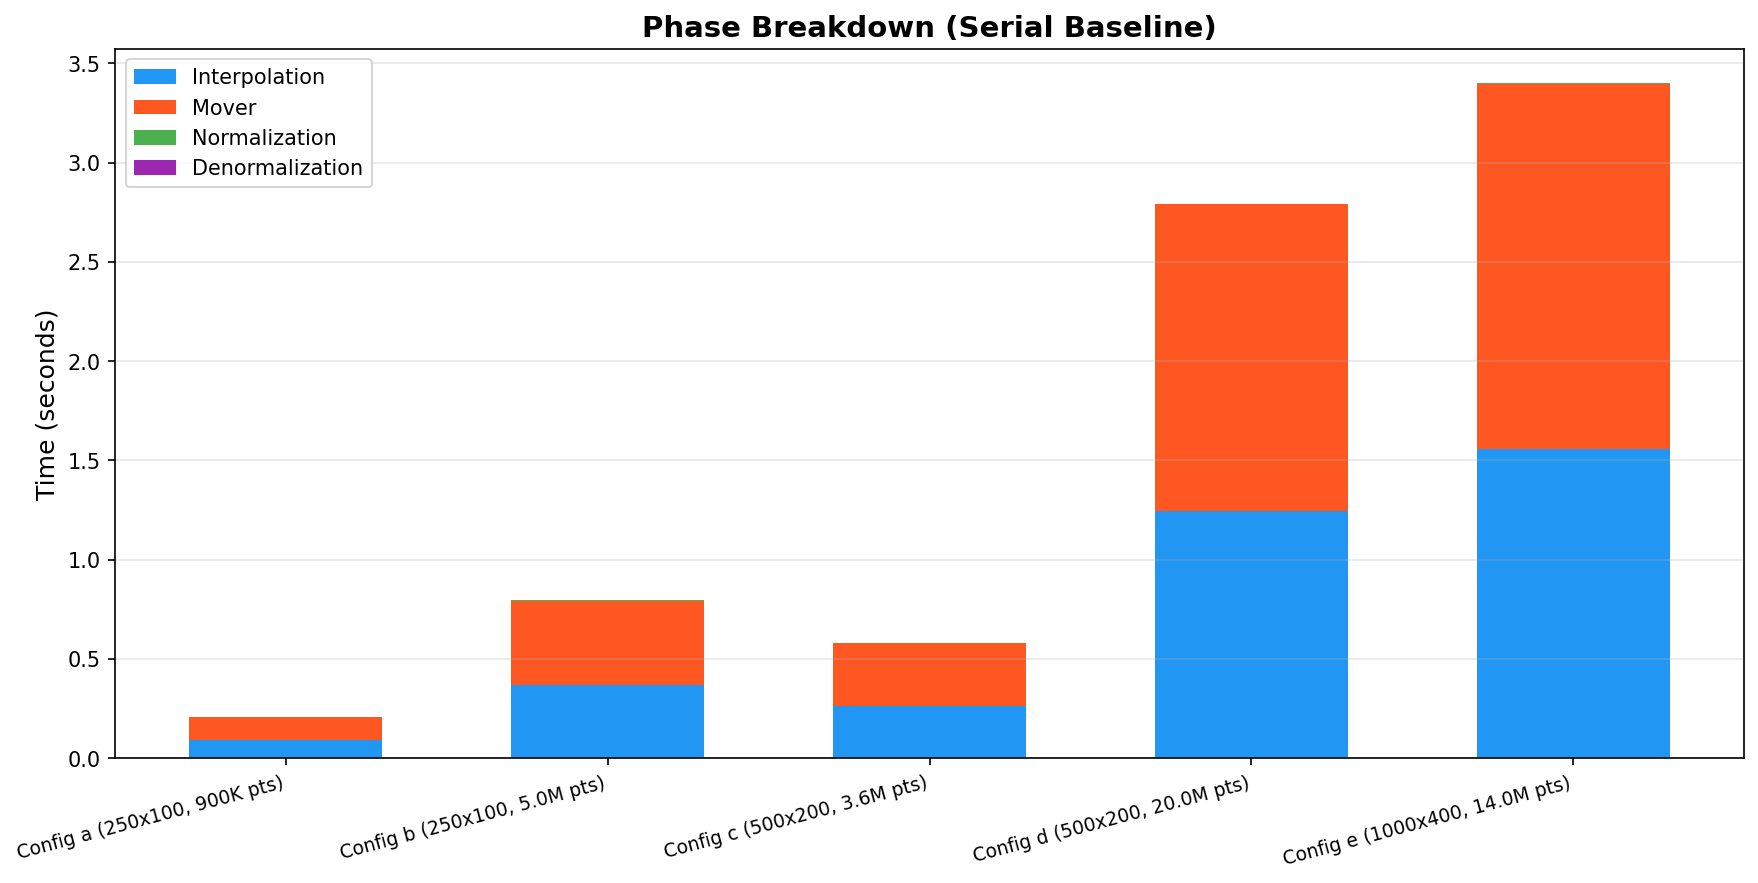
\includegraphics[width=0.85\textwidth]{results/cluster/phase_breakdown.png}
\caption{Phase-level breakdown of execution time on HPC Cluster. The mover phase
dominates serial execution; it parallelizes better than the interpolation phase.}
\label{fig:a7_phase_cluster}
\end{figure}

\subsection{Lab PC Results (Windows)}

\begin{figure}[H]
\centering

\includegraphics[width=0.85\textwidth]{results/lab/speedup_vs_cores.png}
\caption{Speedup vs Number of Threads (Lab PC, Assignment~07). Scaling plateaus beyond
8 threads; oversubscription on the 8-core machine.}
\label{fig:a7_lab_speedup}
\end{figure}

\begin{figure}[H]
\centering

\includegraphics[width=0.85\textwidth]{results/lab/execution_time_vs_cores.png}
\caption{Execution Time vs Number of Threads (Lab PC, Assignment~07).}
\label{fig:a7_lab_time}
\end{figure}

\begin{figure}[H]
\centering

\includegraphics[width=0.85\textwidth]{results/lab/parallel_efficiency_vs_cores.png}
\caption{Parallel Efficiency vs Number of Threads (Lab PC, Assignment~07).}
\label{fig:a7_lab_eff}
\end{figure}

\begin{figure}[H]
\centering

\includegraphics[width=0.85\textwidth]{results/lab/phase_breakdown.png}
\caption{Phase-level breakdown of execution time on Lab PC (Windows).}
\label{fig:a7_phase_lab}
\end{figure}

\subsection{Per-Configuration Analysis --- HPC Cluster}

\begin{figure}[H]
\centering
\begin{subfigure}[b]{0.48\textwidth}
    
\includegraphics[width=\textwidth]{results/cluster/config_a_analysis.png}
    \caption{Config a (250$\times$100, 0.9M pts)}
\end{subfigure}
\hfill
\begin{subfigure}[b]{0.48\textwidth}
    
\includegraphics[width=\textwidth]{results/cluster/config_b_analysis.png}
    \caption{Config b (250$\times$100, 5.0M pts)}
\end{subfigure}

\vspace{0.5cm}

\begin{subfigure}[b]{0.48\textwidth}
    
\includegraphics[width=\textwidth]{results/cluster/config_c_analysis.png}
    \caption{Config c (500$\times$200, 3.6M pts)}
\end{subfigure}
\hfill
\begin{subfigure}[b]{0.48\textwidth}
    
\includegraphics[width=\textwidth]{results/cluster/config_d_analysis.png}
    \caption{Config d (500$\times$200, 20M pts)}
\end{subfigure}

\vspace{0.5cm}

\begin{subfigure}[b]{0.48\textwidth}
    
\includegraphics[width=\textwidth]{results/cluster/config_e_analysis.png}
    \caption{Config e (1000$\times$400, 14M pts)}
\end{subfigure}

\caption{Per-configuration analysis (Execution Time + Speedup) on HPC Cluster ---
Assignment~07.}
\label{fig:a7_per_config_cluster}
\end{figure}

\subsection{Per-Configuration Analysis --- Lab PC}

\begin{figure}[H]
\centering
\begin{subfigure}[b]{0.48\textwidth}
    
\includegraphics[width=\textwidth]{results/lab/config_a_analysis.png}
    \caption{Config a (250$\times$100, 0.9M pts)}
\end{subfigure}
\hfill
\begin{subfigure}[b]{0.48\textwidth}
    
\includegraphics[width=\textwidth]{results/lab/config_b_analysis.png}
    \caption{Config b (250$\times$100, 5.0M pts)}
\end{subfigure}

\vspace{0.5cm}

\begin{subfigure}[b]{0.48\textwidth}
    
\includegraphics[width=\textwidth]{results/lab/config_c_analysis.png}
    \caption{Config c (500$\times$200, 3.6M pts)}
\end{subfigure}
\hfill
\begin{subfigure}[b]{0.48\textwidth}
    
\includegraphics[width=\textwidth]{results/lab/config_d_analysis.png}
    \caption{Config d (500$\times$200, 20M pts)}
\end{subfigure}

\vspace{0.5cm}

\begin{subfigure}[b]{0.48\textwidth}
    
\includegraphics[width=\textwidth]{results/lab/config_e_analysis.png}
    \caption{Config e (1000$\times$400, 14M pts)}
\end{subfigure}

\caption{Per-configuration analysis (Execution Time + Speedup) on Lab PC --- Assignment~07.}
\label{fig:a7_per_config_lab}
\end{figure}

% ============================================================
% SECTION A7-6: ANALYSIS AND QUESTIONS
% ============================================================
\section{A7: Analysis and Questions}

\subsection{Q1: Pseudocode and Illustrative Diagram}

\subsubsection{Pseudocode}

\begin{lstlisting}[style=pseudocode, caption={Pseudocode for Assignment 07 parallel PIC loop}]
READ points from input.bin (once)
ALLOCATE mesh_value[GRID_Y x GRID_X]

FOR iter = 0 TO Maxiter-1:

  /* PHASE 1: INTERPOLATION (Scatter: particle -> grid) */
  IF T * G_SIZE * 8 < CACHE_THRESHOLD:
    // Thread-local path
    SINGLE: allocate/reuse thread-local grids
    EACH THREAD: MEMSET local_grid
    PARALLEL FOR (static) over particles:
      IF void -> skip
      Compute cell (i,j), weights -> local_grid += weights
    PARALLEL FOR (static) over grid cells:
      mesh[k] = SUM_t local[t][k]       // parallel reduction
  ELSE:
    // Atomic path (large grids)
    PARALLEL FOR (static) over particles:
      IF void -> skip
      ATOMIC: mesh[idx]   += w00, mesh[idx+1] += w10, ...

  /* PHASE 2: NORMALIZATION */
  min_val = +INF;  max_val = -INF
  PARALLEL FOR reduction(min, max) over grid cells:
    min_val = min(min_val, mesh[k])
    max_val = max(max_val, mesh[k])
  PARALLEL FOR over grid cells:
    mesh[k] = 2*(mesh[k]-min_val)/(max_val-min_val) - 1

  /* PHASE 3: MOVER (Gather: grid -> particle) */
  PARALLEL FOR (static) over particles:
    IF void -> skip
    Compute cell (i,j), bilinear weights
    Fi = mesh[4 neighbors] dot weights (READ-ONLY)
    x += Fi*dx;  y += Fi*dy
    IF outside [0,1]x[0,1] -> mark void

  /* PHASE 4: DENORMALIZATION */
  PARALLEL FOR over grid cells:
    mesh[k] = (mesh[k]+1)*(max_val-min_val)/2 + min_val

OUTPUT mesh_value to Mesh.out
PRINT timing per phase + total voids
\end{lstlisting}

\subsubsection{Illustrative Diagram}

\begin{figure}[H]
\centering
\fbox{\parbox{0.9\textwidth}{
\textbf{Iteration Loop ($\times$Maxiter): Four Parallel Phases}

\medskip
\begin{tabular}{|c|c|c|}
\hline
\textbf{Phase} & \textbf{Pattern} & \textbf{Race Condition?} \\
\hline
1. Interpolation & Scatter (particle$\to$grid) & Yes $\to$ thread-local/atomic \\
2. Normalization & Grid reduction + scale  & No (reduction clause) \\
3. Mover         & Gather (grid$\to$particle) & No (read grid; write own fields) \\
4. Denormalization & Grid scale             & No \\
\hline
\end{tabular}

\medskip
\textbf{Adaptive Strategy:}\\
\quad$T \times G \times 8 < 20$ MB $\Rightarrow$ thread-local grids + parallel reduction\\
\quad$T \times G \times 8 \geq 20$ MB $\Rightarrow$ \texttt{omp atomic} on shared grid

\medskip
\textbf{Data Flow:} Input.bin $\rightarrow$ [Interp] $\rightarrow$ [Norm] $\rightarrow$ [Mover] $\rightarrow$ [Denorm] $\rightarrow$ Mesh.out
}}
\caption{Illustrative diagram of the four-phase parallel PIC pipeline (Assignment~07)}
\label{fig:a7_diagram}
\end{figure}

% -----------------------------------------------------------
\subsection{Q2: Parallel Approach and Race Condition Handling}

\textbf{Approach: Adaptive Hybrid (Thread-Local Grids + Atomics)}

\begin{itemize}
    \item \textbf{Interpolation (scatter) --- Phase 1}: The only phase with potential race
          conditions, since multiple particles may update the same grid cell simultaneously.
          We use an \textbf{adaptive strategy}:
          \begin{itemize}
              \item \textit{Thread-local for small/medium grids} ($T \times G \times 8 < 20$~MB):
                    Each thread accumulates into its own private grid; a parallel reduction
                    merges them. Zero contention in the hot path.
              \item \textit{Atomics for large grids} ($T \times G \times 8 \geq 20$~MB):
                    \texttt{\#pragma omp atomic} on the shared grid. With large grids,
                    contention per cell is low ($\approx\!35$ particles/cell), making atomics
                    efficient.
          \end{itemize}

    \item \textbf{Normalization --- Phase 2}: OpenMP \texttt{reduction(min:...) reduction(max:...)}
          handles the global min/max safely. The scaling pass is independently parallel.

    \item \textbf{Mover (gather) --- Phase 3}: Inherently race-free. Each particle reads
          from the shared (read-only) grid and writes only to its own fields.

    \item \textbf{Denormalization --- Phase 4}: Independent element-wise scaling; plain
          \texttt{parallel for}.
\end{itemize}

\begin{table}[H]
\centering
\begin{tabular}{lll}
\toprule
\textbf{Strategy} & \textbf{Advantage} & \textbf{Disadvantage} \\
\midrule
Atomic (all grids)      & Simple, low memory & CAS overhead, slow for small grids \\
Thread-local (all grids) & Zero contention   & Cache thrash for large grids \\
\textbf{Adaptive hybrid} & Best of both      & Slightly more code complexity \\
\bottomrule
\end{tabular}
\end{table}

% -----------------------------------------------------------
\subsection{Q3: Plots}

All plots are presented in Section~A7-5 ``Performance Visualisations''. Summary:
\begin{itemize}
    \item Figure~\ref{fig:a7_cluster_speedup}: Speedup vs Cores (HPC Cluster)
    \item Figure~\ref{fig:a7_cluster_time}: Execution Time vs Cores (HPC Cluster)
    \item Figure~\ref{fig:a7_cluster_eff}: Parallel Efficiency (HPC Cluster)
    \item Figure~\ref{fig:a7_phase_cluster}: Phase breakdown (HPC Cluster)
    \item Figure~\ref{fig:a7_per_config_cluster}: Per-config analysis (HPC Cluster)
    \item Figures~\ref{fig:a7_lab_speedup}--\ref{fig:a7_per_config_lab}: Lab PC counterparts
\end{itemize}

% -----------------------------------------------------------
\subsection{Q4: Parallel Efficiency and Scalability}

Parallel efficiency $E(T) = S(T)/T \times 100\%$ (Table~\ref{tab:a7_efficiency}).

\textbf{Key observations (HPC Cluster):}
\begin{itemize}
    \item \textbf{Config~a} maintains $\approx\!100\%$ efficiency up to 4 threads and
          \textbf{79\%} at 16 threads --- excellent for a small-grid problem.
    \item \textbf{Config~b} achieves \textbf{10.82$\times$ speedup} at 16T ($\approx\!68\%$
          efficiency) despite the additional normalization/mover overhead of Assignment~07.
    \item \textbf{Config~e} drops to \textbf{16\%} efficiency at 16T. At 8T the adaptive
          strategy switches to atomics (total local memory = $8 \times 401\text{K} \times 8
          = 25.7$~MB $>$ 20~MB threshold), reducing the interpolation speedup sharply.
    \item Configs with a \textbf{high particles-to-grid ratio} (b, d) scale better because
          parallel work in the mover and interpolation phases dominates over the
          normalization/reduction overhead.
\end{itemize}

% -----------------------------------------------------------
\subsection{Q5: Maximum Speedup Achieved}

\begin{table}[H]
\centering
\caption{Maximum speedup achieved on HPC Cluster --- Assignment~07}
\label{tab:a7_max_speedup}
\begin{tabular}{clccc}
\toprule
\textbf{Config} & \textbf{Points} & \textbf{Serial (s)} & \textbf{Best Parallel (s)} & \textbf{Max Speedup} \\
\midrule
a & 0.9M  & 0.2074 & 0.0163 & \textbf{12.71$\times$} @ 16T \\
b & 5.0M  & 0.7943 & 0.0734 & \textbf{10.82$\times$} @ 16T \\
c & 3.6M  & 0.5801 & 0.0577 & \textbf{10.05$\times$} @ 16T \\
d & 20.0M & 2.7910 & 0.3535 & \textbf{7.90$\times$}  @ 16T \\
e & 14.0M & 3.4020 & 1.3098 & \textbf{2.60$\times$}  @ 16T \\
\bottomrule
\end{tabular}
\end{table}

Config~a achieves the best overall speedup (12.71$\times$) owing to its small grid fitting
entirely in per-thread caches during both interpolation and mover phases.

% -----------------------------------------------------------
\subsection{Q6: Explanation of Speedup and Observations}

\textbf{Why we achieve good speedup:}
\begin{enumerate}
    \item \textbf{Adaptive interpolation} eliminates the choice between cache thrash and atomic
          slowness. Thread-local grids give zero contention for configs a--d.
    \item \textbf{The mover is embarrassingly parallel}: each particle reads from a shared
          (read-only after normalization) grid and writes only its own position --- ideal
          for \texttt{schedule(static)}.
    \item \textbf{Persistent thread-local storage}: allocated once, reused across all 10
          iterations, eliminating per-iteration malloc/free overhead.
    \item \textbf{Precomputed reciprocals} (\texttt{inv\_dx}, \texttt{inv\_dy}) turn
          division into multiplication in both the interpolation and mover kernels.
\end{enumerate}

\textbf{Why speedup is sub-linear:}
\begin{enumerate}
    \item \textbf{Reduction overhead}: Merging $T$ local grids is $O(G \times T)$ extra
          work.
    \item \textbf{Sequential normalization min/max}: Even with \texttt{reduction}, small
          synchronization barriers exist.
    \item \textbf{Memory bandwidth saturation}: At 8+ threads, all threads compete for
          DRAM bandwidth. The 20M-point array ($\approx\!480$~MB) far exceeds any cache.
    \item \textbf{Config e anomaly (8T)}: Total thread-local memory ($8\times3.2$~MB$=
          25.6$~MB) exceeds the 20~MB threshold, switching to atomics, which is slower
          than the thread-local path.
\end{enumerate}

% -----------------------------------------------------------
\subsection{Q7: Optimization with Unlimited HPC Resources}

\begin{enumerate}
    \item \textbf{GPU Offloading (CUDA/OpenCL)}: The interpolation and mover loops are
          ideal for GPU. Thousands of CUDA cores can process millions of particles
          simultaneously. The grid fits in GPU L2 cache for small/medium configs.
    \item \textbf{MPI + OpenMP Hybrid}: Distribute particles across nodes via MPI domain
          decomposition; use OpenMP within each node. A final \texttt{MPI\_Reduce} merges
          per-node grids.
    \item \textbf{SIMD Vectorization (AVX-512)}: Restructure the particle array from
          AoS (\texttt{\{x,y,void\}}) to SoA (\texttt{x[], y[], void[]}) to enable
          processing 8 particles per instruction.
    \item \textbf{NUMA-Aware Allocation}: Use first-touch policy or \texttt{numactl} to
          place each thread's local grid on its local NUMA node, minimizing remote memory
          latency on multi-socket systems.
    \item \textbf{Active Particle Compaction}: Periodically compact void particles to the
          end of the array, eliminating branch mispredictions from void checks and
          improving cache line utilization.
    \item \textbf{Cache-Aware Particle Sorting}: Sort particles by grid cell after each
          mover step to maintain spatial locality in the next interpolation.
\end{enumerate}

% -----------------------------------------------------------
\subsection{Q8: Load Imbalance and Performance Bottlenecks}

\subsubsection{Load Imbalance}

\begin{itemize}
    \item \textbf{Interpolation}: Random particle distribution $\Rightarrow$
          \texttt{schedule(static)} divides work evenly --- good balance.
    \item \textbf{Mover}: After each iteration some particles become void (60--1254 out
          of millions). Void skip is a single branch prediction; imbalance is negligible.
          If imbalance became severe (e.g., $>10\%$ void), \texttt{schedule(dynamic)}
          could help, but dispatch overhead exceeds benefits at our particle counts.
\end{itemize}

\subsubsection{Performance Bottlenecks}

\begin{enumerate}
    \item \textbf{Mover dominance (serial)}: The mover accounts for 50--61\% of serial
          time because it reads grid values \textit{and} updates particle positions
          (read + write per particle).
    \item \textbf{Adaptive switch overhead}: For config~e at 8T+ the atomic path is
          used; atomic CAS loops add $\sim$10--20 cycles per update vs.\ zero for the
          thread-local path.
    \item \textbf{Memory bandwidth}: The 20M-point particle array ($480$~MB) far exceeds
          any cache level. At 8+ threads, DRAM bandwidth becomes the bottleneck.
    \item \textbf{Thread-local grid memory}: Config~e at 16T: $16\times3.2$~MB = 51.2~MB,
          exceeding L3 cache. The threshold switches to atomics, but throughput still
          suffers.
\end{enumerate}

% -----------------------------------------------------------
\subsection{Q9: Alternative Approach}

\subsubsection{Alternative 1: Pure Atomic Operations}

\begin{lstlisting}[caption={Pure atomic approach for interpolation}]
#pragma omp parallel for schedule(static)
for (int p = 0; p < NUM_Points; p++) {
    if (points[p].is_void) continue;
    // ... compute weights ...
    #pragma omp atomic
    mesh_value[idx]   += w00;
    #pragma omp atomic
    mesh_value[idx+1] += w10;
    // ... two more atomics ...
}
\end{lstlisting}

\begin{itemize}
    \item \textbf{Pros}: No extra memory, no reduction phase, simpler code.
    \item \textbf{Cons}: CAS-loop overhead ($\approx\!10$--20 cycles/atomic), cache-line
          ping-pong at high thread counts.
    \item \textbf{Best for}: Large grids where contention is naturally low
          ($<50$ particles/cell).
\end{itemize}

\subsubsection{Alternative 2: Color-Based Domain Decomposition}

Partition grid cells into a \textit{checkerboard} (red/black or 4-color). In each color
pass, all cells of that color have no adjacent conflicts, so particles assigned to those
cells can be updated without synchronization.

\begin{itemize}
    \item \textbf{Pros}: No extra memory, no reduction phase, no atomics.
    \item \textbf{Cons}: Requires spatial particle sorting (preprocessing); $\geq 4$
          sequential passes reduce effective parallelism.
\end{itemize}

\textbf{Our adaptive hybrid is superior} because it requires no pre-sorting and avoids
the coloring penalty while adapting dynamically to grid size.

% -----------------------------------------------------------
\subsection{Q10: Data Structures and OpenMP Approaches for Performance}

\subsubsection{Approach 1: Structure of Arrays (SoA)}
Replace the AoS layout \texttt{struct \{double x, y; int is\_void;\}} with separate
arrays \texttt{double x[], y[]; int void[]}. Enables AVX-512 SIMD of 8 doubles at a
time, eliminates struct padding, and improves prefetch efficiency.

\subsubsection{Approach 2: Spatial Hashing}
Bin particles into a hash table keyed by grid cell. Process each cell's particles
independently, enabling conflict-free updates without thread-local copies.

\subsubsection{Approach 3: Tree Reduction for Thread-Local Grids}
Merge local grids in $O(\log T)$ passes (pair-wise reduction tree) instead of the flat
$O(T)$ sequential loop. Reduces reduction time from $O(G \cdot T)$ to
$O(G \cdot \log T)$, beneficial at very high thread counts ($T \geq 32$).

\subsubsection{Best Choice for This Problem}
The \textbf{adaptive thread-local + parallel flat reduction} is optimal for our
configurations because:
\begin{itemize}
    \item Grid size $G \ll N$ for configs a--d, so reduction overhead is negligible
          relative to interpolation/mover work.
    \item Thread-local grids fit in L3 cache for configs a--d, yielding zero-contention
          scatter.
    \item The mover is embarrassingly parallel with no added data structure requirement.
\end{itemize}

% -----------------------------------------------------------
\subsection{Q11: Phase-by-Phase Performance Analysis}

Table~\ref{tab:phase_breakdown} shows the serial phase breakdown. Key findings:

\begin{itemize}
    \item \textbf{The mover is the serial bottleneck} (50--61\% of total time) because
          it performs both grid reads (gather: 4 cells per particle) and particle writes
          (2 position updates + void check).
    \item \textbf{Interpolation is 39--49\% of serial time}: despite writing to 4 cells
          (scatter), the computation per particle is identical to the mover's gather
          computation.
    \item \textbf{Normalization/denormalization are negligible} ($<$1\% of total) because
          they loop only over $G \ll N$ grid cells.
    \item \textbf{In the parallel version, the mover parallelizes better} (embarrassingly
          parallel, no reduction), so the interpolation-with-reduction becomes the
          \textit{relative} bottleneck at high thread counts. This is visible in
          Figure~\ref{fig:a7_phase_cluster}.
\end{itemize}

% ============================================================
% SECTION A7-7: CONCLUSION
% ============================================================
\section{A7: Conclusion}

We successfully extended the parallel interpolation (Assignment~06) into a full
particle-in-cell simulation pipeline (Assignment~07) using OpenMP. Key results:

\begin{itemize}
    \item \textbf{Correctness verified}: Output \texttt{Mesh.out} matches the reference
          \texttt{Test\_Mesh.out} exactly (zero entry-wise differences) for all thread
          counts tested.
    \item \textbf{Maximum speedup of 12.71$\times$} achieved on the HPC cluster for
          Config~a at 16 threads.
    \item \textbf{Adaptive interpolation strategy} avoids the pitfalls of both pure
          thread-local (cache thrash at large grids) and pure atomic (CAS overhead at
          small grids), delivering near-optimal performance across all five
          configurations.
    \item \textbf{The mover phase parallelizes extremely well} (embarrassingly parallel)
          and contributes significantly to total speedup.
    \item \textbf{Config~e} is the hardest to scale due to its large grid size triggering
          the atomic fallback and causing higher reduction overhead. With GPU offloading or
          a distributed MPI+OpenMP approach, near-linear scaling would be achievable even
          for this configuration.
\end{itemize}

\end{document}

